\documentclass{article}


% *** *** *** %
\usepackage{indentfirst}
\usepackage{graphicx}
\usepackage{authblk}
\usepackage{url}
\usepackage{tikz}
\usetikzlibrary{shapes,shadows,calc}
\usepackage{subfigure}
\usepackage{microtype}
\def\tm{\leavevmode\hbox{$\rm {}^{TM}$}} %\tm
\newcommand{\cs}{C\slash S}
% *** *** *** %


\begin{document}

\title{Egal Car: A Peer-to-Peer Car Racing Game Synchronized Over Named Data Networking}
\author{Zening Qu \thanks{quzening@remap.ucla.edu}}
\affil{UCLA REMAP}
\author{Jeff Burke \thanks{jburke@remap.ucla.edu}}
\affil{UCLA REMAP}

\date{\today}
\maketitle

\begin{abstract}
Multiplayer online games require synchronization mechanisms to maintain game state consistency among all the players. This project explored the use of the emerging collection synchronization primitives in Named Data Networking (NDN) to easily synchronize a simple multiplayer car racing game, Egal Car, in a peer-to-peer fashion.  The game was based on a Unity game engine demo application. To implement the experiment, C\# bindings usable in Unity were built for PARC's CCNx library, including the new Sync protocol. The impacts of the unordered nature of default CCNx synchronization and unreliable delivery in basic Interest/data exchange were explored.  This work will inform an upcoming exploration of how to build a more extensive multiplayer role-playing game using NDN.  
\end{abstract}

%============================================================================%
\section{Introduction}
\label{introduction}

One of the most important differences between a multiplayer online game (MOG) and its single-player counterpart is that the former requires a shared virtual world and game state consistency across network-connected players. Consistency ensures that all players in the shared virtual world are able to form a correct understanding of it and have the desired orientation to it. For example, a car racing game should provide each player with a \emph{consistent} view of all the cars' positions in real-time, and there should be no collision between any two views. 

For a MOG with players distributed over a wide geographic area, delivery of game state updates usually relies on packets transmitted over the Internet.  This paper documents the implementation of a simple MOG over a possible future Internet architecture, Named Data Networking (NDN)~\cite{Jndn}. In particular, it explores the use of new collection synchronization mechanisms now available in NDN.  As discussed below, NDN names data instead of hosts. It has inherent multicast data delivery, caching, content signing, and collection synchronization capabilities that could provide substantial benefits for multiplayer games and distributed simulations. As it relates to these applications, NDN can be regarded as a new datagram delivery service, an alternative to TCP\slash IP. However, NDN also has the potential to impact game or simulation design and conceptualization, and to assist implementation and improve performance. 

By creating a MOG on the NDN testbed, NDN's impact on MOG design and implementation was explored.  The simple MOG described here, Egal Car, provides preliminary experience to inform the creation of a more sophisticated game and a test for C\# libraries usable with the Unity game engine. 

Egal Car is a 3D car racing game with a highly detailed track and scenery. Each player has control over one car, which can increase in speed, slow down and alter direction. The cars can collide with each other and with fences along the track. All car movements are simulated by the game's physics engine. Like in other racing games, each player's goal is to win the race.  Egal Car is adapted from an open source game template, Unity  Car Tutorial~\cite{UnityCar}. This template provides the necessary graphics and physics modules, but it is a single-player offline game.  The project designed and engineered this network module, a synchronization mechanism with the needs of this car racing game in mind. 

Following are descriptions of the design choices and details of the implementation. Section~\ref{ndnbackground}~introduces NDN principles and facts that may inspire MOG design. Sections~\ref{architecture}~through~\ref{implementation}~discuss MOG design, using Egal Car as a main example.


%============================================================================%
\section{NDN Background}
\label{ndnbackground}

NDN retrieves data based on application-defined names rather than host addresses. To retrieve data, the consumer must know the name, instead of the data's location (host address) as in IP.  NDN communication uses two packet types: \emph{Interest} and \emph{Data}. An Interest packet is issued by the receiver to express what set of data is needed. A Data packet is published by the sender in response to an Interest. Both Interest and Data packets use names to identify the data being exchanged (see figure~\ref{img:packet_types}). An Interest is ``satisfied'' when a Data packet is received with a Content Name that falls within the prefix of the Content Name in the Interest packet. For more detail, see ~\cite{Jndn}. 

\begin{figure}
\begin{center}
\includegraphics[width=0.7\textwidth] {image/packet_types}
\caption{Interest packet and Data packet}
\label{img:packet_types}
\end{center}
\end{figure}

% introduce CCNx and Sync
This project explores higher-level features being made available in NDN for collection synchronization.  There are a few general purpose synchronization protocols under development. Among them is the CCNx\footnote{CCNx is an implementation of NDN and an open source project by Xerox PARC.} Synchronization Protocol (CCNx Sync) ~\cite{CCNxSync}, which synchronizes collections of named data under a given name prefix. The research examines how it can be used to support game synchronization, as described above. The results show that CCNx Sync can provide significant benefits to MOG development by handling many of the low-level details for maintaining consistency across different instances of the networked game.

%============================================================================%
\section{Architecture}
\label{architecture}

%As described above, a simple game with a limited number of interacting objects was selected, and an approach for peer-to-peer synchronization was designed. 
There are two main classes of MOG network architectures, client\slash server (\cs) and peer-to-peer (P2P). In \cs~architectures, all clients directly communicate with a central server, which is the only authorized source of game state updates (see figure~\ref{cs}). In P2P architectures, peers (clients) communicate with each other directly, and each peer computes the latest game state on its own (see figure~\ref{p2p}).  Typical implementations in major multiplayer online games appear to follow the \cs~model using connectionless protocols such as UDP.\footnote{Connection-oriented protocols such as TCP can also be used; however, others have shown that such protocols may result in severe performance degradation. Thus, they are rarely used by MOGs~\cite{Fgame}.}

\begin{figure} 
\centering  
\subfigure[\cs]  
{  
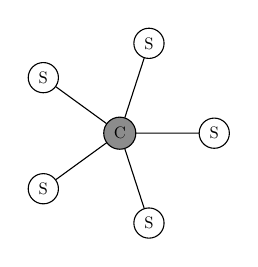
\begin{tikzpicture} [scale=0.6, transform shape]
\tikzstyle{every node}=[draw,shape=circle];
\node [fill = gray!90] (v0) at (0:0) {C};
\node (v1) at ( 0:2) {S};
\node (v2) at ( 72:2) {S};
\node (v3) at (2*72:2) {S};
\node (v4) at (3*72:2) {S};
\node (v5) at (4*72:2) {S};
\draw (v0) -- (v1) % star
(v0) -- (v2)
(v0) -- (v3)
(v0) -- (v4)
(v0) -- (v5);
\end{tikzpicture}
\label{cs}
}  
\subfigure[P2P]  
{  
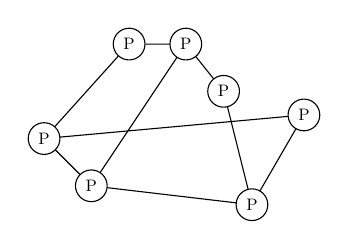
\begin{tikzpicture} [scale=0.6, transform shape]
\tikzstyle{every node}=[draw,shape=circle];
\node (v0) at (0, 2) {P};
\node (v1) at (1, 1) {P};
\node (v2) at (1.8, 4) {P};
\node (v3) at (3, 4) {P};
\node (v4) at (4.4, 0.6) {P};
\node (v5) at (3.8, 3) {P};
\node (v6) at (5.5, 2.5) {P};
\draw (v0) -- (v1)
(v0) -- (v2)
(v0) -- (v6)
(v4) -- (v5)
(v1) -- (v4)
(v2) -- (v3)
(v3) -- (v5)
(v4) -- (v6)
(v3) -- (v1);
\end{tikzpicture}
\label{p2p}
}
\caption{\cs~architecture and P2P architecture}
\end{figure}

Despite its rarity in implementing major multiplayer online games, it is generally agreed that P2P approaches outperform \cs~in scalability, latency and robustness~\cite{Fgame, Scheating}. However, in typical IP implementations, P2P game network architectures face significant performance limitations. For example, due to limited deployment of IP multicast~\cite{Fgame}, they have higher bandwidth requirements than \cs~games. A common scenario is that every player wants to exchange packets with all other players. For example, in Egal Car, every player would benefit from knowing the positions of all the other players' cars. When this is implemented by direct communications between all the players, it would lead to an enormous amount of traffic. In a \cs~network, on the other hand, the traffic is alleviated because the centralized server plays the role of an ``information aggregator'', and each player communicates with all other players by exchanging packets with the server only. 

The lack of a central authority in P2P architectures is a more fundamental limitation, making player and update authentication more difficult and cheating easier~\cite{Scheating}. 

P2P architecture was chosen for this project's prototype, Egal Car. 
NDN makes a P2P-based multiplayer game much more feasible. Because NDN has multicast data delivery content caching built-in, it can substantially reduce network traffic in one-to-many scenarios like P2P state distribution.  
%%The star topology of \cs~architectures cannot fully exploit NDN's communication model.  
Game state can be obtained by many peers from one or more sources on the network using NDN's inherent multicast and caching. 
Furthermore, because NDN secures every data packet rather than securing the communication channel as currently done in SSL, cryptographic authentication of signed content objects can be used to alleviate the issues related to cheating.  
%The project team plans to explore how NDN features can be used to alleviate these issues in the upcoming year.  

The choice of game architecture greatly impacts other network module design decisions, such as the synchronization mechanism. For example, in \cs~architectures, clients might send certain types of user inputs to the server, and the server would compute the result of the inputs. A client would not compute the result on its own because it has neither the right to compute the next game state nor the information that is sufficient to do so. Instead of claiming, ``I am three blocks away from my last position now'', a client would only tell the server, ``I want to move three blocks to the north-east'', and let the server confirm its new position. On the contrary, with P2P architectures, every peer has the right and the information to compute its own next game state, assuming all the players can maintain consistent game state.
%(The resulting challenges to maintain game consistency across peers can be significant and will be the topic of upcoming work.) 
This gives more freedom to individual players in deciding what to send to other peers. A peer can choose to send out user inputs, as a client would in \cs~architecture, or choose to send out the result of its inputs and ask the other peers to update their information. The later approach has been adopted in Egal Car for synchronizing information about each car's position (see section~\ref{assetsynchronization}).


%============================================================================%
\section{Synchronization}
\label{synchronization}

In this project, asset synchronization and state synchronization are approached differently to explore the requirements and constraints of slowly and quickly changing data.  These two approaches may be combined in future work. 

Below, (1) data are classified as either \emph{assets} or \emph{states}; 
(2) data to be synchronized are identified; and
(3) different experimental approaches for asset and state synchronization are defined.



%-------------------------------------------------------------------------------------------------------------------------------------%
\subsection{Namespace}
\label{namespace}

The data were identified within a namespace design that accounts for the assets and relevant state of the single-player application used as the basis for Egal Car.  According to Knutsson et al.~\cite{Upen}, a virtual world is typically comprised of immutable elements (terrain) and mutable elements (players, non-player characters, mutable objects, mutable landscape). The immutable elements are to be installed before gameplay begins, at level changes, and other significant moments. The properties, instantiation and deletion of the mutable elements are to be synchronized in real time. 

In Egal Car, there are three types of data: 
\begin{enumerate}
\item the terrain, track, and car graphics, which are immutable, unchanging across peers and thus do not need synchronization;  
\item asset creation and deletion, controlled by player login and logout; and 
\item synchronized state, which includes properties of the assets as well as global game state.\footnote{State nodes do not come in and out of existence on their own, but are created and deleted with an asset or game.  Conceptually, global game state can be considered properties of a root node.}  
\end{enumerate}
The time between asset updates (player login and logout, in this case) may be measured in seconds or even minutes, but the state changes more regularly and rapidly in the cases being considered. In Egal Car, a car's position, for example, tends to be calculated for every video frame. The time between a car position state update and its successor is usually measured in milliseconds. It is relatively easy to predict the desired frequency of state updates, as this is often guided by game applications frame rates and perceived interaction latency.

Figure~\ref{img:namespace} illustrates Egal Car's namespace, composed of three trees. Each node contains one or more name components. Each path that starts from the root denotes a name.\footnote{The brackets \texttt{< >} around name components denote that they will be substituted with ``real'' values at run time. For example, when Egal Car is executing the actual name might be \texttt{/ndn/ucla.edu/apps/EgalCar/AliceCar/123456/transform/position}.}

\begin{figure}
\begin{center}
\begin{subfigure} [Repository Tree]
{
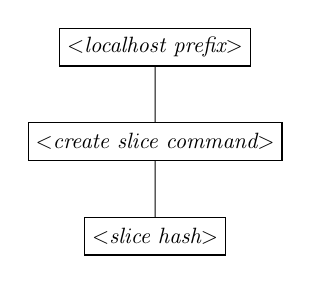
\begin{tikzpicture} [scale=0.8, transform shape]
    \tikzstyle{every node}=[minimum size=6mm,
				% The border:
      				 ,
     				 draw=black,
      				% The filling:
				font=\itshape
					]
    \node {$<$localhost prefix$>$}
        child { node {$<$create slice command$>$} 
        		child{ node {$<$slice hash$>$} }
        }
    ;
\end{tikzpicture}
\label{img:repotree}
}
\end{subfigure}

\vspace{30pt}
\begin{subfigure} [Discovery Tree]
{
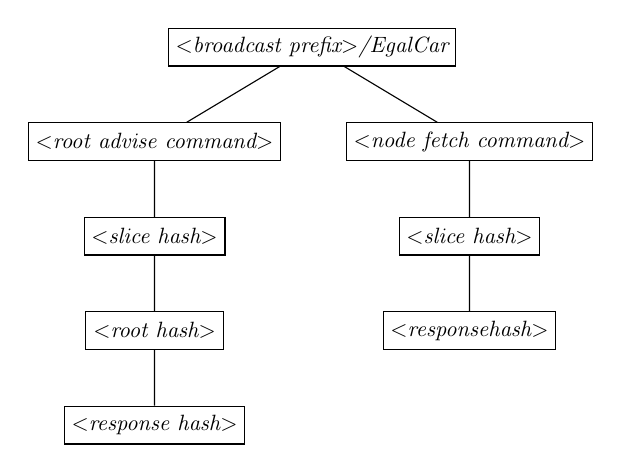
\begin{tikzpicture} [scale=0.8, transform shape]
    \tikzstyle{every node}=[align = center, minimum size=6mm,
				% The border:
      				,
     				 draw=black,
      				% The filling:
				font=\itshape
					]
    \tikzstyle{level 1} = [sibling distance=50mm]
    \node {$<$broadcast prefix$>$/EgalCar}
        child { node {$<$root advise command$>$} 
        		child { node {$<$slice hash$>$} 
			child { node {$<$root hash$>$} 
				child { node {$<$response hash$>$}} }
		}
        }
        child { node {$<$node fetch command$>$}
        		child { node {$<$slice hash$>$} 
			child { node {$<$responsehash$>$} }
		}
        }
    ;
\end{tikzpicture}
\label{img:discovery}
}
\end{subfigure}

\vspace{30pt}
\begin{subfigure} [Object Tree]
{
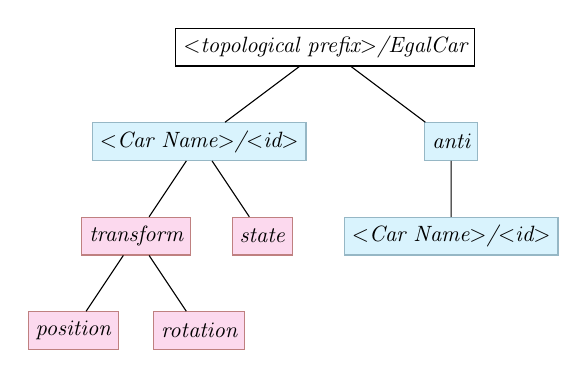
\begin{tikzpicture} [scale=0.8, transform shape,
				state/.style={
				% The shape:
				rectangle,
				% The size:
      				minimum size=6mm,
				% The border:
      				,
     				 draw=red!50!black!50,
      				% The filling:
				fill = magenta!15,
				%top color=white,
				%bottom color=red!50!black!20, % and something else at the bottom % Font
				font=\itshape
    				},
				asset/.style={
				% The shape:
				rectangle,
				% The size:
      				minimum size=6mm,
				% The border:
      				,
     				 draw=cyan!50!black!50,
      				% The filling:
				fill = cyan!15,
				%top color=cyan!50!black!20,
				%bottom color=cyan!50!black!20, % and something else at the bottom % Font
				font=\itshape
    				},
				default/.style={
				% The shape:
				rectangle,
				% The size:
      				minimum size=6mm,
				% The border:
      				,
     				 draw=black,
      				% The filling:
				font=\itshape
    				},
				]
    \tikzstyle{every node} = [align=center]
   % \tikzstyle{asset} = [fill=cyan!15]
   % \tikzstyle{state} = [fill=magenta!15]
   % \tikzstyle{event} = [fill=orange!15]
    \tikzstyle{level 1} = [sibling distance=40mm]
    \tikzstyle{level 2} = [sibling distance=20mm]
    \node [default] {$<$topological prefix$>$/EgalCar}
        child { node [asset] {$<$Car Name$>$/$<$id$>$} 
		child { node [state] {transform} 
			child{ node [state] {position} }
			child{ node [state] {rotation} }
		}
		child { node [state] {state} }
        }
         child{ node [asset] {anti}
        		child { node [asset] {$<$Car Name$>$/$<$id$>$}}
        }
    ;
\end{tikzpicture}
\label{img:gametree}
}
\end{subfigure}
\caption{The NDN namespace of Egal Car.}
\label{img:namespace}
\end{center}
\end{figure}

The object tree (figure~\ref{img:gametree}) shows all asset and state names, in blue and red respectively. The root node is composed of the \texttt{<topological prefix>}, where game data can be published, and the game's name, \texttt{EgalCar}. Our instantiation of the application for testing used a \texttt{<topological prefix>} of \texttt{/ndn/ucla.edu/apps}. Other NDN games would use their own values for \texttt{EgalCar} and \texttt{<topological prefix>}. 

In the figure, the leftmost child of the root shows the namespace for cars in the game. Nodes using this convention (and their children) are dynamically created when a player joins in the game. Since Egal Car is a MOG, there will be more than one \texttt{<Car Name>/<id>} node, as players discover each other (see~\ref{assetsynchronization}). The \texttt{<id>} component, which will be substituted by a random number during run-time, is designed in case there is a name collision in \texttt{<Car Name>}. The right child of the root node is used to indicate that a certain player (car) has quit or disconnected. The \texttt{anti} node and its child nodes are all assets. The remaining nodes are state names, and they are synchronized differently than assets.

As stated in Section~\ref{ndnbackground}, CCNx Sync can be used to aid multiplayer game development. Egal Car uses its basic features to support asset synchronization, game discovery and player discovery, given the proper namespace design.
To do so, two other trees (the Repository Tree and the Discovery Tree) are needed in the namespace.  The Repository Tree is a namespace used by each game peer to communicate with its local CCNx repository, where asset data is stored and synchronized by CCNx Sync. \texttt{<localhost prefix>}, the root node of the Repository Tree, confines the communication scope to localhost. The Discovery Tree is the collection of names used by CCNx Sync. Its root node is similar to that of the Game Tree except that it has a broadcast scope (\texttt{<broadcast prefix>}). Since CCNx Sync is used for ``discoveries'', it is important that its packets be broadcast to reach all potential data publishers that may appear anywhere in the network. More details of the Repository Tree and the Discovery Tree follow in Section~\ref{assetsynchronization}.

%-------------------------------------------------------------------------------------------------------------------------------------%
\subsection{Asset Synchronization}
\label{assetsynchronization}

% CCNx Sync
Asset synchronization, specifically player entry and exit, is implemented through the discovery of new objects in the sync tree. The process is discussed in some detail here as Sync is a relatively new primitive in the NDN architecture. 

When an instance of the application is initialized for the first time, a \emph{slice} is defined in the local repository~\cite{CCNxCS} that defines the content objects to be synchronized. At that time, two names are provided to the Sync mechanism: the \texttt{<broadcast prefix>} and the \texttt{<topological prefix>}. The first defines CCNx Sync's broadcast namespace to use in communicating with other Sync daemons, while the second is the common prefix of every name in the slice. 

An application informs its local repository about the creation of a slice by issuing a start write Interest for the slice configuration object. The name used in this process is \texttt{<localhost prefix>/<create slice command>/<slice hash>}. \texttt{<localhost prefix>} confines the packet within the same node; \texttt{<create slice command>} claims the command type; \texttt{<slice hash>} is the SHA-256 hash of the slice configuration object and is used as the name of the slice in the Discovery Tree.

Once the slice is created, CCNx Sync broadcasts \emph{Root Advise} Interests periodically in the \texttt{<broadcast prefix>}. Root Advise Interests have names of the form \texttt{/<root advise command>/<slice hash>/<root hash>}. The \texttt{<slice hash>} identifies the particular collection of names to be synchronized.  The \texttt{<root hash>} is a hashed digest of a peer's slice. 

So, to participate in a given game, an Egal peer will have that game's \texttt{<slice hash>} in its Root Advise Interest.  Other peers running the same application recognize that peer  because they share a \texttt{<slice hash>}.

A peer's collection of game assets is represented by its \texttt{<root hash>}. If this \texttt{<root hash>} is the same as that of everyone else's \texttt{<root hash>}, then all peers are in sync. If it is not the same, the other peers would respond to the peer's Root Advise Interest with a Data packet named \texttt{/<root advise command>/<slice hash>/<root hash>/<response hash>}. CCNx Sync uses \emph{Node Fetch} command and normal Interest/Data packet exchange to then reconcile differences in the collection among peers, updating the repositories to be consistent.

To announce the creation of a new player (car) to the network, a content object named \texttt{<topological prefix>/EgalCar/<Car Name>/<id>} is published by the player's game instance into its local repository. By using \texttt{<topological prefix>}, this content object becomes part of the slice managed by CCNx Sync. The data of this content object are some configuration information of the car (initial position, 3D model's name, player information, etc.). As other peers learn about the newcomer through CCNx Sync, they use the configuration data to instantiate a 3D car model in the given position, and they mark it with the given player information. 

When a player quits, it writes an \emph{anti-asset} into its own repository. This provides confirmation of object deletion.  (Note that the CCNx repository does not support per-object deletion.)  The anti-asset's name would be \texttt{<topological prefix>/EgalCar/anti/<Car Name>/<id>}, in which the \texttt{<Car Name>} and \texttt{<id>} represent the car that belongs to the quitting player. With CCNx Sync, synchronizing anti-assets is the same as synchronizing assets. Peers that learn about the anti-asset destroy the corresponding avatar in their game world. If a player is forced to quit, due to network failure for example, there is no chance to write the anti-asset. In this case, the anti-asset would be written by other peers who remain connected. 

\subsubsection{Unordered, reliable synchronization}

CCNx Sync provides unordered data synchronization, i.e. it may discover assets that are created later before discovering assets that are created earlier.  In Egal Car, assets are independent of each other, and there is no causal relationship between asset updates as long as there is an application strategy to know when to begin the car race. Thus CCNx Sync can be used as-is. 
Future work will consider the tradeoffs between the unordered synchronization strategy, which works in the limited case of Egal Car, and contemporary ordered approaches (\cite{Chandy, Bryant, Flockstep, Csync, Doptbkt}) for other game types. These ordered synchronization algorithms trade off delay for ordering, either holding every peer's turn to wait for the correct packet to arrive, or performing a rollback when disordering is detected. These ordered synchronization strategies will be needed for updates that are correlated, but they are not necessary in the Egal Car. 

Although asset synchronization is unordered, it does need to be reliable. As an example, Alice and Bob must be known by all other peers regardless of potential packet losses.  NDN, similar to IP, only provides best-effort datagram delivery. The reliability in asset synchronization is achieved by CCNx Sync, as the synchronization routine periodically broadcasts Root Advise Interests throughout the lifetime of the game.  As soon as any difference between any repositories is detected, 
%%their \texttt{<root hash>} would differ, 
CCNx Sync will reconcile the difference.

%--------------------------------------------------------------------------------------------------------------------------------------%
\subsection{State Synchronization}
\label{statesynchronization}

In Egal Car, state is a snapshot of a variable (property) associated with an asset or the game instance. In the application namespace, state updates are versioned content objects that are children of a uniquely named asset.  For example, state updates of Alice's car use this name \texttt{.../<AliceCar>/<id>/transform/\\position/<version>} to refer to Alice's position, where \texttt{<version>} is a timestamp. As with asset creation and deletion described above, the states of Alice and Bob will not affect each other: \texttt{.../<AliceCar>/<id>/transform/position} updates will not cause \texttt{.../<BobCar>/<id>/transform/position} to change.  Note that this does not relate to the case when Alice and Bob interact with each other. Such interactions lead to players' state change. A new model for these interactions is being developed for future work. 

\subsubsection{Ordered, unreliable updates}
Egal Car state updates are snapshots rather than change logs.  For consistency of visual rendering, they should be ordered, with the most recent state update 
representing the object state, % \emph{overwrite} for a given peer 
and undelivered state updates ignored.
State synchronization does not need to be reliable as long as there is either no player interaction (global state is deterministic based on player state input) or a facility is available to periodically confirm overall state. 

Therefore unlike asset synchronization, it is unnecessary, or even undesirable, to use reliable game synchronization algorithms for state synchronization in the Egal Car scenario.  When a state update is lost, there is no reason to hamper the game's pace to wait for retransmission in order to achieve an ordered state update or to perform rollbacks, as the latest state is what the gameplay needs.  (Again, this is for the limited case of no permanent modification to the asset's behavior happening because of a state update.)

Instead of CCNx Sync, NDN's Interest-Data exchange is used directly for state synchronization in Egal Car.  Each player's instance issues Interests for the state updates that it wants to follow, and maintains a \emph{timestamp floor} for each state update series. For example, Alice follows Bob's position by periodically expressing an Interest in \texttt{.../<BobCar>/<id>/transform/position}. 
%% This is done to limit broadcast traffic that would be generated by using the CCNx sync mechanism as done for assets.
To this Interest, NDN nodes may respond with any data matching its prefix, so the Interests must be constructed to obtain the latest child for a given game object prefix.  This is achieved by setting selectors in Interest packets appropriately: The \emph{rightmost child selector} is set, and an \emph{exclusion filter} is used to exclude data with versions less than or equal to the timestamp floor. The result is that a player may miss some state updates if a newer one has already been published, but whatever state reaches the player will be at least later than the previous one received.\footnote{Note that because any NDN node may answer an Interest with cached data, the state that is received may not be \emph{globally} the latest state, but will at least be later than the timestamp floor given in the exclusion filter.}


\subsubsection{Traffic optimizations}

State synchronization is what generates the largest amount of traffic in most MOGs~\cite{Upen}.  In many cases every player wishes to follow the state of all other players in real time, and every player is expected to exchange several data per second\footnote{Larger environments may incorporate some type of partitioning if there are a very large number of players.} In a P2P network of $n$ players, the number of packets being sent for state synchronization per second ($N$) can be estimated by \begin{math}N = xf\bar{h}n(n-1)\end{math}, where $x$ is the number of packets necessary for a state exchange, which is usually greater or equal to two. $f$ is the frequency of state exchange defined by the game application. $\bar{h}$ is the average number of hops that packets must travel. In IP networks, $\bar{h}$ equals the average distance (in hops) between peers, as each peer is both a data receiver and a data sender. In NDN networks, $\bar{h}$ will be significantly smaller because most Interest and Data packets do not need to travel from each data publisher to all receivers.  Interests for the same data aggregate on their way towards the data publisher, Data packets propagate along a multicast tree, and are cached at each hop~\cite{Jndn}.  Many Interests need to travel only a few hops to be satisfied by data from cache, or to be combined with an identical Interest.  This reduces the average travel distance of packets, and should make NDN games generate much less traffic than IP games.

Some optimization can be done to the game application's packet contents to further reduce the traffic generated by state synchronization. In Egal Car, the \texttt{state} node in the Game Tree (see figure~\ref{img:gametree}) is designed for such optimization. The \texttt{state} object is a summary of other state updates (\texttt{transform/position} and \texttt{transform/rotation}), and is synchronized instead of its siblings.


%============================================================================%
\section{Implementation}
\label{implementation}

Egal Car is developed with Unity, one of the ten most prominent game engines~\cite{unityrank}. It is adapted from Unity's single-player car race tutorial~\cite{UnityCar}. The tutorial's gameplay has been left intact, and the project's network module makes the tutorial a MOG.  After implementation, the synchronization for a small number of peers (2-3) was tested, and game play was evaluated. 

The network modules builds on the CCNx libraries, as illustrated in figure~\ref{peerarchitecture}. A CCNx daemon named \texttt{ccnd} provides basic Named Data Networking support, such as sending and receiving Interest and Data packets.  Asset synchronization requires a local repository, such as CCNx's \texttt{ccnr}, which manages read\slash write requests to the repository. Finally, CCNx Sync is used to \emph{manage} repository contents (see section~\ref{synchronization}). 

The Egal network module is where asset and state synchronization is implemented. It contains \texttt{C\#} scripts for Unity and two \texttt{C} libraries (see figure~\ref{img:networkmodule}). The network scripts implement the project's synchronization mechanism by invoking functions provided by the Egal library and the CCNx library. CCNx library contains programming interfaces given by the CCNx project. Egal library is based on CCNx library, but it provides some convenient functions for synchronization. The \emph{InteropServices} of the \emph{.NET Framework} are used to invoke \texttt{C} functions from \texttt{C\#} and vice versa.


%********************%
\def\tboxl[#1,#2,#3,#4,#5]#6{%
  \node[draw,, minimum height=#1, minimum width=#2, %
  inner color=white, outer color=white, color=black] (#4) at #5 {}; %
  \node[anchor=#3,inner sep=2pt] at (#4.#3) {#6};%
}

%-----#1 name of the node, #2 coordinate, #3 label
\def\entity[#1,#2]#3;{
  \node[draw,,color=black,fill=white,rounded corners=3] (#1) at #2 {#3};
}

%-----#1 from node, #2 to node, #3 specification of a node (label), #4
%-----dashed, or other parameters for draw
\def\isaedge[#1,#2,#3,#4];{ 
  \draw[<->,color=black!20!black,#4,fill=white] (#1) -- #3
  (#2);  
}

%-----ABoxes
%-----#1 height, #2 width, #3 aspect, #4 name of the node, #5
%-----coordinate, #6 label   
\def\aboxr[#1,#2,#3,#4,#5]#6{%
  \node[draw, cylinder, alias=cyl, shape border rotate=90, aspect=#3, %
  minimum height=#1, minimum width=#2, outer sep=-0.5\pgflinewidth, %
  color=black, left color=white, right color=white, middle
  color=white] (#4) at #5 {};%
  \node at #5 {#6};%
  \fill [white] let \p1 = ($(cyl.before top)!0.5!(cyl.after top)$), \p2 =
  (cyl.top), \p3 = (cyl.before top), \n1={veclen(\x3-\x1,\y3-\y1)},
  \n2={veclen(\x2-\x1,\y2-\y1)} in (\p1) ellipse (\n1 and \n2); }

%-----#1 height, #2 width, #3 name of the node, #4
%-----coordinate, #5 label
\def\kbbox[#1,#2,#3,#4,#5]#6{
        \draw[dashed] node[draw,color=gray!50,minimum
        height=#1,minimum width=#2] (#4) at #5 {}; 
        \node[anchor=#3,inner sep=2pt] at (#4.#3)  {#6};
}
\begin{figure}
\begin{center}
  \begin{tikzpicture} [scale=1.2, transform shape]
    \small
    \kbbox[144,120,south,Peer1,(0,1.25)] {Peer};
    \tboxl[40,100,north,t1,(-0,2.7)] {$Egal Car$};
    \entity[Module,(-0,2.4)] {$Network Module$};
   % \tboxl[12,40,north,t1,(1.3,2.4)] {$Egal$};
    \aboxr[20,50,1.4,Repo,(-0.6,1.2)] {$Repository$};
    \entity[Sync,(-0.6,0.4)] {$CCNx Sync$};
    \entity[Daemon,(-0,-0.5)] {$CCNx Daemon$};
    \isaedge[Module,Repo,,];
    \isaedge[Repo,Sync,,];
    \isaedge[Sync,Daemon,,];
    \draw[<->,color=black!20!black,,,] plot [smooth,tension=1.5] coordinates{(-0,2.17) (1,0.85) (-0,-0.27)};
    \node [cloud, draw,cloud puffs=10,cloud puff arc=120, aspect=2, inner ysep=1em] at (5,-0.5) {network};
   % \kbbox[30,60,south,Peer2,(5,-0.5)] {Peer};
   % \kbbox[30,60,south,Peer3,(4,-1)] {Peer};
     \draw[<->,  thick, color=black!20!black,,,] (1.3,-0.5) -- (3.7,-0.5) node [midway, above] {Interest/Data};
    % \draw[<->,  thick, color=black!20!black,,,] (0.4,-0.5) -- (3,-1) node [midway, below] {Interest/Data};
  \end{tikzpicture}
\caption{CCNx components used by Egal Car.}
\label{peerarchitecture}
\end{center}
\end{figure}

%********************%
\begin{figure}
\begin{center}
  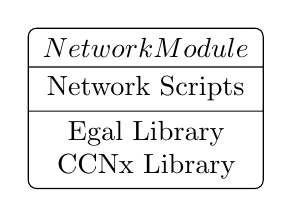
\begin{tikzpicture}
  
%  \node[draw,,minimum height=60,minimum width=100,color=black,fill=white,rounded corners=3] (Rounded) at (0,0) {};
%  \node[anchor=north,inner sep=2pt] at (Rounded.north) {$Network Module$};
%  \entity[Script,(0,-0.2)] {$Network Scripts$};
%  \entity[Egal,(-0.8,-0.8)] {$Egal$};
%  \entity[CCNx,(0.8,-0.8)] {$CCNx$};
  
  \node[rectangle split, rectangle split parts=3, draw, text width=2.75cm, align=center, rounded corners=3]
        {$Network Module$
        \nodepart{second}
        Network Scripts
        \nodepart{third}
        Egal Library \\
        CCNx Library}; 
    
  \end{tikzpicture}
\caption{The network module's relationship to other libraries.}
\label{img:networkmodule}
\end{center}
\end{figure}
%********************%


%============================================================================%
\section{Discussions and Future Work}
\label{futurework}

% interactions
Egal Car is a relatively simple MOG prototype, and the project's synchronization mechanism was easy to develop using NDN collection synchronization. With Egal Car, assets are independent of each other, and they have no explicit interaction. This is why unordered or unreliable synchronization strategies can be applied to the game without hurting its consistency.  

The project's synchronization mechanism does not apply to game genres that have numerous user interactions, such as role-playing games (RPG) and real-time strategy games (RTS). Inter-user interactions would lead to state changes and even asset changes. A new model is needed to describe interactions, and a new synchronization strategy would have to be designed (or chosen) to meet its requirements. Studying a new model and synchronization strategy is planned for the future.

% scale
Egal Car is not an appropriate test for scaling, as it has few asset updates and a limited number of players. To evaluate whether, or by how much, P2P games would be more scalable on NDN than on IP in general, new test cases would need to be implemented. Building a multiplayer online role-playing game with more sophisticated asset and state interaction is planned, as is the study of scaling through actual play and simulation.

% cheating
Finally, of special importance to P2P games is the research of game security and cheating-prevention. Since network security in NDN is approached quite differently from that of traditional IP networks\footnote{In NDN, the emphasis is on \emph{securing the data} rather than \emph{securing the channel} as currently done in SSL, for example. Cryptographic authentication of signed content objects and encryption of private data are the two main approaches to be explored in the next game project.}, numerous updates to authentication and anti-cheating mechanisms are expected.


%============================================================================%
\section{Conclusions}
\label{conclusions}

This project developed straightforward synchronization mechanisms for simple car racing games over NDN, using the CCNx sync protocol and bindings created for the Unity game engine. The mechanism was implemented in a prototype game, \emph{Egal Car}, and organized into an open-source synchronization library, \emph{Egal}, to support future NDN game developers. Also explored was the workflow of NDN-based multiplayer game development. Collection synchronization approaches using named data appear to hold promise for streamlining development and performance of multiplayer online games and distributed simulation, especially in terms of simplifying development and deployment of peer-to-peer architecture.  For simple games like Egal Car, where updates are independent of each other, default unordered and unreliable synchronization strategies can be used to deliver expected interactivity without hurting consistency.   Future work will be required to meet the synchronization requirements of  more complex online virtual environments.   


%============================================================================%
\section{Acknowledgements}
\label{acknowledgements}

Thanks to Alex Horn and Alessandro Marianantoni of REMAP for their help testing the sample application, and to Lixia Zhang for feedback on the architecture.    

%============================================================================%
\bibliographystyle{plain}
\bibliography{sample}

\end{document}



